%                                                                 aa.dem
% AA vers. 8.2, LaTeX class for Astronomy & Astrophysics
% demonstration file
%                                                       (c) EDP Sciences
%-----------------------------------------------------------------------
%
%\documentclass[referee]{aa} % for a referee version
%\documentclass[onecolumn]{aa} % for a paper on 1 column  
%\documentclass[longauth]{aa} % for the long lists of affiliations 
%\documentclass[rnote]{aa} % for the research notes
%\documentclass[letter]{aa} % for the letters 
%\documentclass[bibyear]{aa} % if the references are not structured 
% according to the author-year natbib style

%
\documentclass{aa}
\usepackage{graphicx}
%%%%%%%%%%%%%%%%%%%%%%%%%%%%%%%%%%%%%%%%
\usepackage{txfonts}
%%%%%%%%%%%%%%%%%%%%%%%%%%%%%%%%%%%%%%%%
\usepackage{hyperref}
\pdfoutput=1
\usepackage{amsfonts}
\usepackage{amsmath}
\usepackage{amssymb}
\usepackage{xcolor}
\usepackage{enumitem}
\usepackage{graphicx}
\usepackage{gensymb}
\usepackage{fancyhdr}
\usepackage{times}
\usepackage{ulem}
%\usepackage{caption}
\usepackage{subcaption} 
\usepackage{float} 
\usepackage{color}
 

\definecolor{purple}{RGB}{76, 0,153}
\newcommand{\ch}[1]{{\color{purple}{#1}}}
\newcommand{\bg}[1]{\textcolor{orange}{#1}}

\newcommand{\dd}{{\rm d}}
\newcommand{\br}[1]{\left( #1 \right)}
\newcommand{\bc}[1]{\left\{ #1 \right\}}



\newcommand{\be}{\begin{equation}}  \newcommand{\ee}{\end{equation}}


\begin{document} 

   \title{KiDS-1000 Cosmology: Multi-probe weak gravitational lensing and spectroscopic galaxy clustering constraints}

   \author{Catherine Heymans \inst{1,2}\thanks{Catherine Heymans: heymans@roe.ac.uk} 
   \and Tilman Tr\"oster\inst{1}\thanks{Tilman Tr\"oster: ttr@roe.ac.uk} 
   \and Marika Asgari\inst{1} 
   \and Chris Blake\inst{3}
   \and Hendrik Hildebrandt\inst{2}
   \and Benjamin Joachimi\inst{4}
   \and Chieh-An Lin\inst{1}
   \and Ariel Sanchez\inst{5}
   \and Tilman Tr\"oster\inst{1}
   \and Jan Luca Van den Busch\inst{2}
   \and Angus Wright\inst{2}
   \and the KiDS Collaboration
          }
\institute{Institute for Astronomy, University of Edinburgh, Royal Observatory, Blackford Hill, Edinburgh, EH9 3HJ, UK 
   \and
   Ruhr-Universität Bochum, Astronomisches Institut, German Centre for Cosmological Lensing (GCCL), Universitätsstr. 150, 44801, Bochum, Germany
   \and 
   Centre for Astrophysics \& Supercomputing, Swinburne University of Technology, P.O. Box 218, Hawthorn, VIC 3122, Australia
   \and
   University College London, Gower Street, London WC1E 6BT, UK
   \and
   Max-Planck-Institut f\"ur extraterrestrische Physik, Postfach 1312, Giessenbachstrasse 1, D-85741 Garching, Germany
   %Department of Astrophysical Sciences, Princeton University, 4 Ivy Lane, Princeton, NJ 08544, USA
     % \and
   %Department of Physics, University of Oxford, Denys Wilkinson Building, Keble Road, Oxford OX1 3RH, U.K.
    }
   % Leiden Observatory, Leiden University, Niels Bohrweg 2, 2333 CA Leiden, the Netherlands
 %  \date{Received September 15, 1996; accepted March 16, 1997}

% 5 {} token are mandatory
 
  \abstract{TBD}

 \keywords{gravitational lensing: weak, methods: data analysis, methods: statistical, surveys, cosmology: observations}

   \titlerunning{KiDS-1000: 3x2pt}
   \authorrunning{Heymans, Tr\"oster \& the KiDS Collaboration et al.}
   \maketitle
%
%________________________________________________________________
\section{Introduction}
\label{sec:intro}

Observations of the cosmic microwave background (CMB) have delivered high-precision
constraints for the cosmological parameters of the flat, cold dark
matter and cosmological constant model of the Universe
\citep[$\Lambda$CDM,][]{planck/etal:2018}.  With only six free
parameters, this flat $\Lambda$CDM model provides an exquisite fit to observations of
the anisotropies in the CMB.    The same model predicts a range of
different observables in the present day Universe, including the cosmic expansion rate \citep{weinberg/1972}, and the
distribution of, and gravitational lensing by, large-scale
structures \citep{peebles/1980,bartelmann/schneider:2001,eisenstein/etal:2005}.  
In most cases there
is agreement between the measured cosmological parameters of the flat $\Lambda$CDM model, when comparing those
constrained at the CMB epoch with those constrained through a variety of
lower-redshift probes \citep[see the discussion in][and references
therein]{planck/etal:2018}.   Recent improvements in the statistical
precision of the lower-redshift probes have,
however, revealed some statistically significant differences.  Most
notably a $4.4\sigma$ difference in the value of the Hubble constant,
$H_0$, has been reported using distance ladder estimates in \citet{riess/etal:2019}.  If this difference cannot be
attributed to systematic errors in either, or both, experiment, this result
suggests that the flat $\Lambda$CDM model is incomplete.

Many
extensions have been proposed to reconcile the observed differences between
high- and low-redshift probes \citep[see for
example][]{riess/etal:2016,poulin/etal:2018,divalentino/etal:2020}.  All, however, require
additional components
to the cosmological model that move it even further away from the
standard model of particle physics, a model that already struggles to motivate
the existence of cold dark matter and a cosmological constant.  
As the statistical power of the observations continues to improve, focus has moved to establishing
a full understanding of all systematic errors, and the development of mitigation approaches, 
in preparation for the high-precision `full-sky' imaging and spectroscopic
cosmology surveys of the 2020's \citep[{\it Euclid},][]{laureijs/etal:2011,lsst/etal:2009,DESI/etal:2016}.

In this analysis we present a multi-probe `same-sky' analysis of the
evolution of large-scale structures, using imaging and spectroscopic surveys.
Our first observable is the weak gravitational lensing of background
galaxies by foreground large-scale
structures, 
known as `{\it cosmic shear}'.    Our second
observable is the {\it anisotropic clustering of galaxies} within these
large-scale structures, combining measurements of both redshift-space
distortions and baryon acoustic
oscillations.   Our third observable is the weak gravitational lensing of background
galaxies by foreground galaxies, known as
`{\it galaxy-galaxy lensing}'.   As these three sets of two-point
statistics are analysed simultaneously, this combination of probes
is usually referred to as a `\tttp' analysis. 

Each observable in our multi-probe analysis is subject to systematic
uncertainties.  For a cosmic shear analysis, the observable is a
combination of the true cosmological signal with a low-level signal
arising from the intrinsic alignment of galaxies, as well as potential residual
correlations in the data induced by the atmosphere, telescope and
camera.   The signal can also be scaled by both shear
 and photometric redshift measurement calibration errors
 \citep[see][and references therein]{mandelbaum:2018}.   For a galaxy
   clustering analysis, the observable is the true
   cosmological signal modulated by an uncertain, non-linear and
   evolving, galaxy bias function.  This function maps how
   the galaxies trace the
   underlying total matter distribution \citep[see][and references
   therein]{desjacques/etal:2018}. 
   The cosmological clustering
   also needs to be accurately distinguished from artificial clustering in the galaxy sample,
   arising from potentially uncharacterised inhomogeneities in the target selection \citep[see for example][]{ross/etal:2012}. 
   Finally, the galaxy-galaxy
   lensing analysis is subject to the systematics that impact both the
   cosmic shear and clustering analyses.

   When analysing these
   observables in combination
   the different astrophysical and systematic dependencies allow for some degree of
   self-calibration \citep{bernstein/jain:2004, hu/jain:2004,
     bernstein:2009,joachimi/bridle:2010}.  `Same-sky'
   surveys, in which imaging for weak lensing observables overlaps with
   spectroscopy for anisotropic galaxy clustering measurements,
   also allows for their cross-correlation.  Such a survey design therefore
   presents a robust
   cosmological tool that can calibrate and mitigate systematic and astrophysical
   uncertainties through a series of nuisance parameters.   In
   addition to enhanced control over systematics, this combination of probes
   breaks cosmological parameter degeneracies from each individual
   probe. 
   For a flat $\Lambda$CDM model
   this leads to significantly tighter constraints on the matter fluctuation amplitude 
   parameter, $\sigma_8$, and the matter density parameter, $\Omega_{\rm m}$, whilst also decreasing the
   uncertainty on the recovered dark energy equation of state
   parameter in extended cosmology scenarios \citep{hu/jain:2004,gaztanaga/etal:2012}.
   
   Three variants of a joint `\tttp' analysis have been
   conducted to date.  \citet{vanuitert/etal:2018} present a joint power-spectrum
   analysis of the Kilo-Degree Survey \citep[KiDS,][]{kuijken/etal:2015} with
   the Galaxy And Mass Assembly survey
   \citep[GAMA,][]{liske/etal:2015}, incorporating projected
   angular clustering measurements.   \citet{joudaki/etal:2018}
   present a joint analysis of KiDS with the
   2-degree Field Lensing Survey \citep[2dFLenS,][]{blake/etal:2016}
   and the overlapping area in the Baryon Oscillation Spectroscopic Survey \citep[BOSS,][]{alam/etal:2015}, incorporating
   redshift-space clustering measurements.  \citet{abbott/etal:2018}
   present a joint real-space lensing-clustering analysis of the Dark
   Energy Survey \citep[DES,][]{drlicawagner/etal:2018}, using a high-quality
   photometric redshift sample of luminous red galaxies for their projected
   angular clustering measurements.  
   In all three cases a
   linear galaxy bias model was adopted. 
   
   In this analysis we enhance and build upon the advances of previous `\tttp' studies.   We analyse the most recent KiDS data release \citep[KiDS-1000,][]{kuijken/etal:2019}, more than doubling the
   survey area from previous KiDS studies.   We utilise the full BOSS
   area and the `full-shape' anisotropic clustering measurements of \citet{sanchez/etal:2017},
   incorporating information from both redshift-space distortions
   and the baryon acoustic oscillation as our galaxy clustering probe.   We adopt a non-linear
   evolving galaxy bias model, derived from renormalised perturbation theory
   \citep{crocce/scoccimarro:2006, chan/etal:2012}.  
   We maximise the signal-to-noise in our 
   KiDS-BOSS galaxy-galaxy lensing analysis, 
   by including additional overlapping spectroscopy of BOSS-like galaxies from 2dFLenS.

This paper is part of the KiDS-1000 series.  The KiDS-1000 photometry and imaging is presented in \citet{kuijken/etal:2019}.  The core weak lensing data products are presented and validated in \citet[shear measurements,][]{giblin/etal:inprep},  and  \citet[redshift measurements,][]{hildebrandt/etal:inprep}.   \citet{asgari/etal:inprep} conduct the cosmic shear analysis using a range of different two-point statistics, and \citet{joachimi/etal:inprep} detail the methodology behind our `\tttp'  
   analysis, with a particular focus on pipeline validation and accurate covariance matrices.   In this analysis we constrain the cosmological parameters of the flat $\Lambda$CDM model.   A range of different extensions to the $\Lambda$CDM model are considered in \citet{troester/etal:inprep}, including varying dark energy, neutrino mass, spatial curvature and various modified gravity scenarios \citep{bose/etal:2020}.
   This paper is organised as follows.   We review the data and provide a concise summary of the findings of the KiDS-1000 series of papers in Section~\ref{sec:data}.   
 We present our joint cosmological constraints in Section~\ref{sec:results}, and conclude in Section~\ref{sec:conc}.  Appendices tabulate the galaxy properties (\ref{app:properties}), the adopted cosmological parameter priors (\ref{app:priors}),  and the cosmological parameter constraints (\ref{app:parameter-constraints}).   They also discuss a series of sensitivity tests (\ref{app:sensitivity}), the redundancy, validation and software review for our pipeline (\ref{app:codereview}), and detail the minor analysis additions that were included after the analysis was formally unblinded (\ref{app:unblinding}).


   











   
\section{Data}
\label{sec:data}

\subsection{Surveys:  KiDS, BOSS and 2dFLenS}
\label{sec:surveys}
Summary of \citet{kuijken/etal:2019},  \citet{blake/etal:2016}, \citet{alam/etal:2015}

\subsection{Cosmic Shear}
\label{sec:cosmic_shear}
Summary of \citet{asgari/etal:inprep}

\begin{figure}
        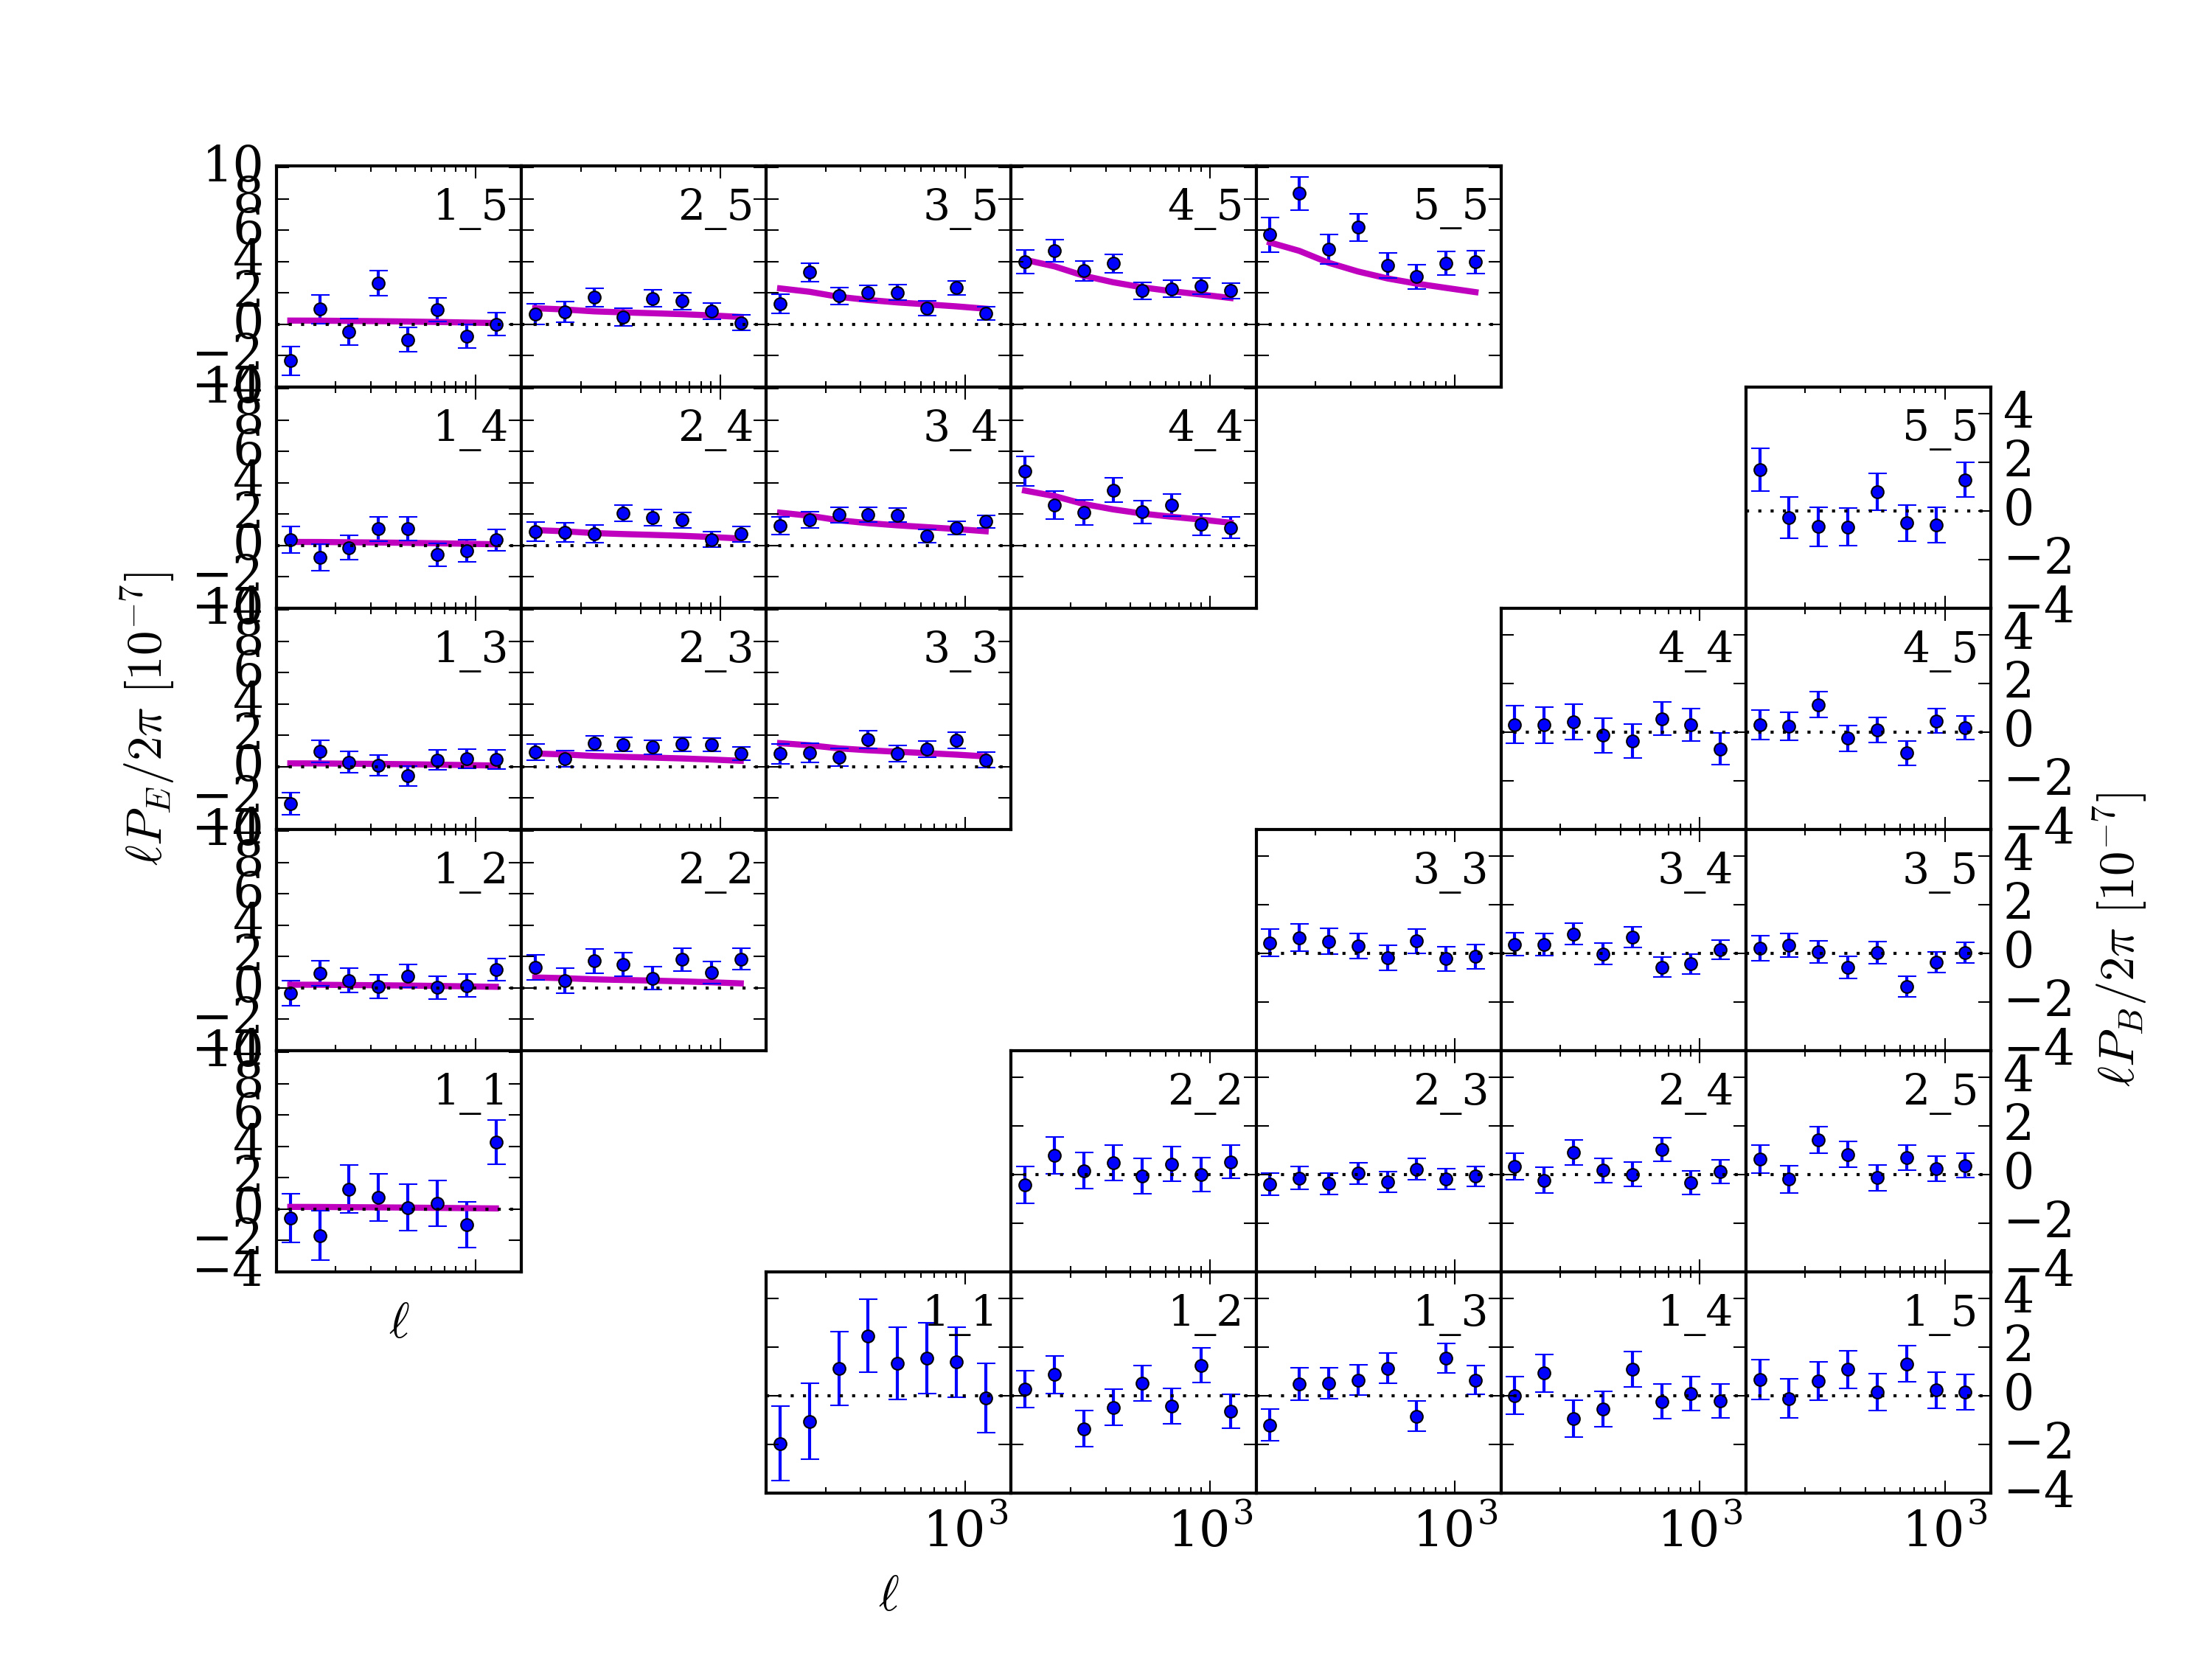
\includegraphics[width=\columnwidth]{Data_Plots/Pkk/Pkk_K1000_2Dbins_v2_goldclasses_Flag_SOM_Fid.png}
        \caption{To do }
        \label{fig:Pkk}
\end{figure}

\subsection{Galaxy-Galaxy Lensing}
\label{sec:GGL}
Summary of Blake et al?

\subsection{Anisotropic Galaxy Clustering}
\label{sec:clustering}
Summary of \citet{sanchez/etal:2017}

\subsection{Covariance}
\label{sec:Cov}
Summary of \citet{joachimi/etal:inprep}


\section{Results}
\label{sec:results}
We present our joint multi-probe constraints on the cosmological parameters of the flat $\Lambda$CDM parameters in Fig.~\ref{fig:cosmology-params}, showing the marginalised posterior distributions for $\sigma_8$, $\Omega_{\rm m}$ and $h$.   Reporting the best-fit MAP with PJ-HPD values for the two parameters that we are most sensitive to, we find (Blind A)
\eqa{
\sigma_8 &= 0.781^{+0.025}_{-0.019} \\ \nonumber
\Omega_{\rm m} &= 0.321^{+0.016}_{-0.010} \\ \nonumber
S_8 &= 0.791^{+0.020}_{-0.012} \, ,
}
where the BOSS galaxy clustering constraints (GC: shown blue), break the $\sigma_8-\Omega_{\rm m}$ degeneracy in the KiDS-1000 cosmic shear constraints (CS: shown pink), resulting in tight constraints on $\sigma_8$ in the combined $3\times2{\rm pt}$ analysis (shown red).   Our constraints can be compared to the marginalised posterior distributions from Planck (shown green), which we discuss in more detail in Sect.~\ref{sec:planck_comp}.

Tabulated constraints for the full set of cosmological parameters are presented in Appendix~\ref{app:parameter-constraints}, quoting our fiducial MAP with PJ-HPD credible intervals, along with the standard marginal posterior mode with M-HPD credible intervals.   We note that the standard quoted marginal mode constraint on $S_8$ is $\sim 10\%$ tighter than the MAP constraint.  As discussed in \citet{joachimi/etal:inprep}, however, this estimate can be easily misinterpreted, yielding systematically low values of $S_8$ in mock data analyses.   This now known bias, can be seen in Fig.~\ref{fig:S8comp}, which compares the MAP constraints (solid) with the marginal (dashed).  

\begin{figure}
	\begin{center}
		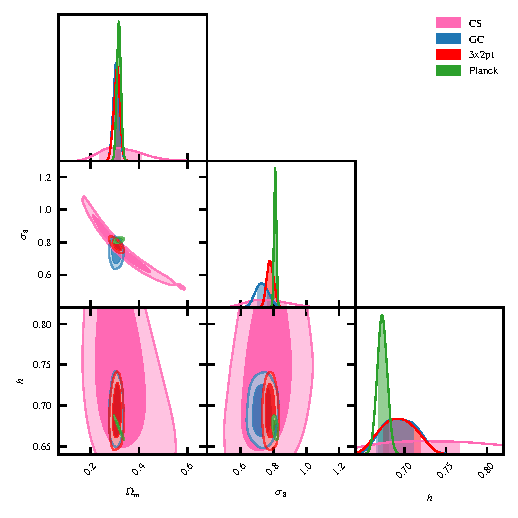
\includegraphics[width=\columnwidth]{Parameter_Plots/cosmology/omegam_sigma8_h_blind_A}
		\caption{Constraints on flat $\Lambda$CDM blind A}
		\label{fig:cosmology-params}
	\end{center}
\end{figure}

We find good agreement between the different probe combinations and single probe $S_8$ constraints, demonstrating internal consistency between the different cosmological probes, in Fig.~\ref{fig:S8comp}.  As forecast by \citet{joachimi/etal:inprep}, the addition of the galaxy-galaxy lensing observable adds very little constraining power, with similar results found for the full $3\times2{\rm pt}$ analysis and the combined cosmic shear and clustering analysis.   This is a result of the significant area of BOSS in comparison to KiDS-1000, and the fact that our lack of an accurate non-linear galaxy bias model prohibits the inclusion of large sections of our galaxy-galaxy lensing data vector, shown in Fig.~\ref{fig:Pgk}.     The addition of the galaxy-galaxy lensing does however serve to moderately tighten constraints on the amplitude of the intrinsic alignment model $A_{\rm IA}$. 

\begin{figure}
	\begin{center}
		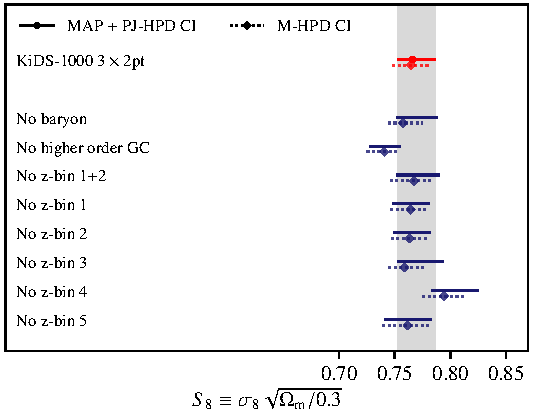
\includegraphics[width=\columnwidth]{Parameter_Plots/systematics/S8_comparison_blindC}
		\caption{Constraints on $S_{8}$ blind C. \TT{Note that the 3x2pt chain has the clustering bug fixed, hence the overall offset.}}
		\label{fig:S8comp}
	\end{center}
\end{figure}

The lower section of Fig.~\ref{fig:S8comp} illustrates the results of a series of sensitivity tests, where we explore how our constraints on $S_8$ change when: we ignore the impact of baryon feedback (the `No baryon' case), fixing $A_{\rm baryon}=3.13$, corresponding to the non-linear matter power spectrum for a dark-matter only cosmology; we limit the analysis to a linear galaxy bias model, setting all higher-order bias terms in Eq.(\ref{eq:pgg}), to zero; when we remove individual tomographic bins from our weak lensing observables.    The only outlier in this series of tests is the linear-bias model, which highlights the importance of accurate non-linear galaxy bias modelling in $3\times2$pt analyses.    This series of tests complements the more detailed KiDS-1000 internal consistency analysis of \citet{asgari/etal:inprep}, and is dissected in Appendix~\ref{app:sensitivity}.

Fig.~\ref{fig:cosmology-params-all} displays the marginalised posterior distributions for an extended set of cosmological parameters.   We find that the constraint on galaxy bias,  $b_1$, in each redshift bin (lower two rows), is more than halved with the addition of the weak lensing data.   This constraint does not arise, however, from the sensitivity of the galaxy-galaxy lensing observable to galaxy bias.  Instead, in this analysis, it is a result of the degeneracy breaking in the $\sigma_8-\Omega_{\rm m}$ plane, tightening constraints in $\sigma_8$ which, for galaxy clustering, is fully degenerate with galaxy bias.  The improved constraints on galaxy bias do not, however, fold through to improved constraints on $h$, which the weak lensing data adds very little information to.

For the majority of the cosmological parameters shown in Fig.~\ref{fig:cosmology-params-all}, the constraints are uninformed by our choice of prior.  The three key exceptions are the spectral index, $n_{\rm s}$, the Hubble parameter, $h$, and the baryon feedback amplitude, $A_{\rm baryon}$.  As noted by \citet{troester/etal:2020}, the BOSS galaxy clustering constraints favour a low value for $n_{\rm s}$, where they find $n_{\rm s} = 0.815 \pm 0.085$.  They conclude that this preference is primarily driven by the amplitude of the large scale clustering signal with $s > 100 \, h^{-1}\, {\rm Mpc}$.  As spurious excess power in this regime could plausibly arise from variations in the stellar density impacting the BOSS galaxy selection function \citep{ross/etal:2017}, we chose to impose an informative prior for $n_{\rm s}$, as listed in Table~\ref{tab:priors}.   This prior does not degrade the overall goodness of fit to the galaxy clustering measurements, and is no more informative than the $n_{\rm s}$ priors that are typically used in weak lensing and clustering analyses \citep[see for example][]{sanchez/etal:2017,abbott/etal:2018}.  We do recognise, however, that this choice of prior serves to reduce the BOSS-only error on $\Omega_{\rm m}$ by roughly a third (see Appendix~\ref{app:priors}).   We note that the galaxy clustering preference for low $n_{\rm s}$ also leads to the joint $3\times2{\rm pt}$ constraint favouring the dark-matter only value for the baryon feedback amplitude $A_{\rm baryon}$.   This preference is not significant however, with all values of $A_{\rm baryon}$ within the prior region, compatible at the $<2 \sigma$ level.   BOSS also provides reasonable constraints on $h$, with our $1\sigma$ constraints on $h$ lying within the $h$-prior.   As the marginal probability at the lower prior edge exceeds 20\% of the peak probability, however, we consider this parameter unconstrained by our analysis.

\begin{figure*}
	\begin{center}
		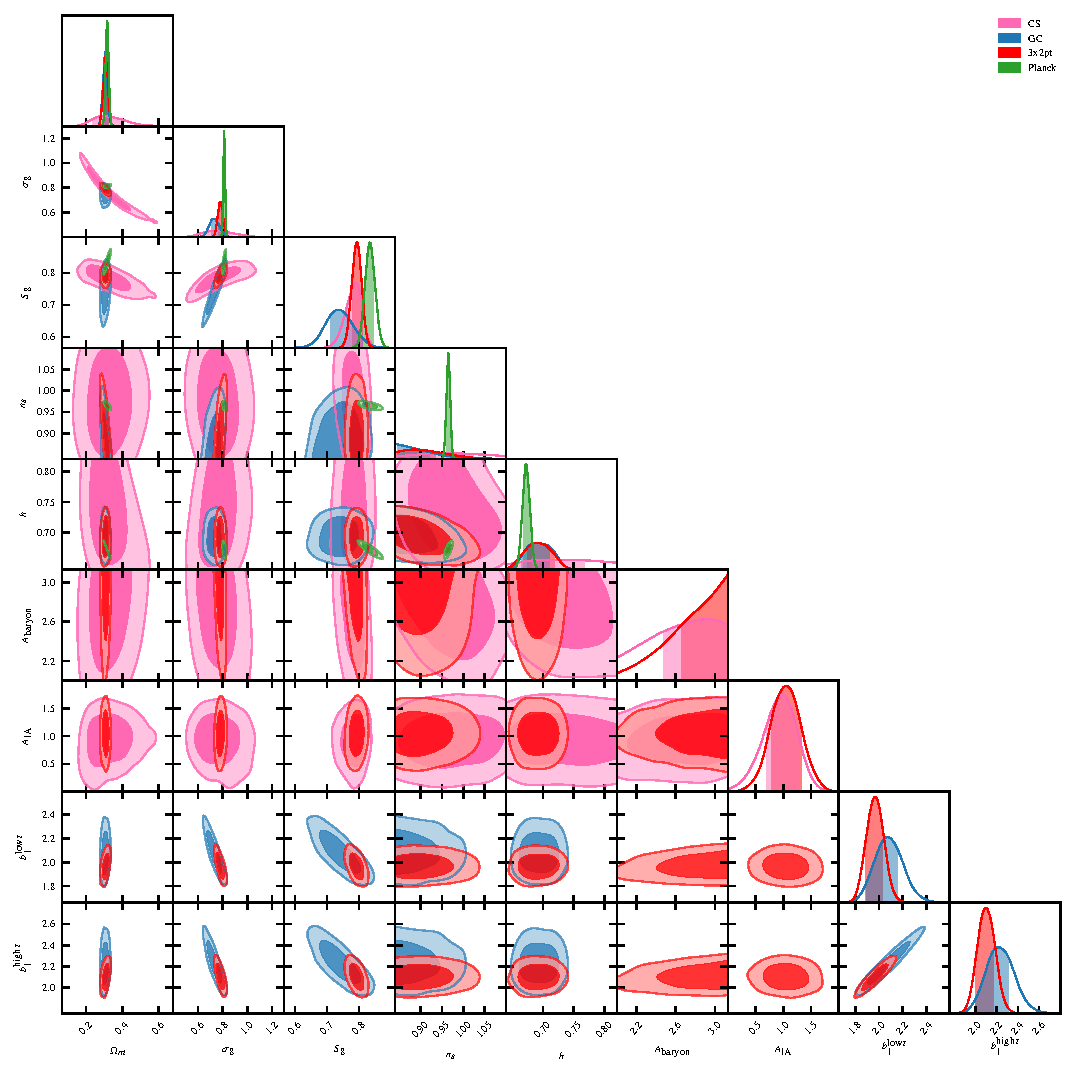
\includegraphics[width=\textwidth]{Parameter_Plots/cosmology/omegam_sigma8_s8_ns_h_a_baryon_a_ia_b1l_b1h_blind_A}
		\caption{Constraints blind A}
		\label{fig:cosmology-params-all}
	\end{center}
\end{figure*}

Table~\ref{tab:goodness-of-fit} records the goodness of fit for each component in our $3\times2$pt analysis.  The effective number of degrees of freedom (DoF) are calculated using the estimator described in section 6.3 of \citet{joachimi/etal:inprep}.   The goodness of fit in all cases is acceptable, but only just.    We are unconcerned by these results, however, given the cosmic shear analysis of \citet{asgari/etal:inprep}, where a different choice in the cosmic shear two-point statistic results in an excellent goodness of fit, with no significant changes in the inferred cosmological parameters.    As such, we could be subject to an unlucky noise fluctuation that particularly impacts the band power estimator in Eq.(\ref{eq:cl_cosmicshear}.  Cautiously inspecting Fig.~\ref{fig:Pkk}, as `$\chi$-by-eye' is particularly dangerous with correlated data points, we nevertheless note a handful of outlying points, for example the low$\ell$-scales in the fifth tomographic bin.   We also note that \citet{giblin/etal:inprep} document a significant but low-level PSF residual systematic in the KiDS-1000 fourth and fifth tomographic bins that was shown to reduce the overall goodness of fit in a cosmic shear analysis, but not bias the recovered cosmological parameters \citep[see also the discussion in][]{amara/refregier:2008}.  Future work to remove these low-level residual distortions are therefore expected to improve the goodness of fit further.

\begin{table}
	\begin{center}
		\caption{Goodness of fit for blind A}
		\label{tab:goodness-of-fit}
\begin{tabular}{lrcl}
    \toprule
    Probe             & $\chi^2$       & DoF       & $p$-value   \\
    \midrule
	CS               & $< 156.3$ & $120-4.5$ & 0.007 \\
	GC               & $< 169.5$ & $168-13$ & 0.202 \\
	CS+GGL           & $187.0$ & $142-7$ & 0.002 \\
	$3\times2$pt            & $367.8$ & $310-20$ & 0.001 \\

    \bottomrule
\end{tabular}
	\end{center}
\end{table}


\subsection{Comparison with Planck}
\label{sec:planck_comp}
This section we will write post-blinding, as until we know which blind it is, it is hard to write.   The short version is A: no tension,  B: oodles of tension,  C: hum.....




\section{Conclusions}
\label{sec:conc}
In this analysis we have presented constraints on the flat $\Lambda$CDM cosmological model by combining observations of gravitational lensing and galaxy clustering to directly probe the evolution and distribution of the large-scale structures in the Universe.    Our survey of the $z \lesssim 1$ low-redshift Universe finds a matter distribution that is less clustered, compared to predictions from the best-fitting $\Lambda$CDM model to early-Universe CMB observations \citep{planck/etal:2018}.  This tendency for low-redshift probes to favour a smoother matter distribution compared to the CMB expectation has persisted since the first large-scale weak lensing survey \citep[CFHTLenS,][]{heymans/etal:2013}, but the significance of this effect has always been tantalisingly around, or below, the $\sim\! 3\,\sigma$ level.   It is therefore unclear if these differences are merely a statistical fluctuation, unaccounted for systematic errors, or a sign of interesting new physics.

Our new result does not lead to a resolution in the matter of statistical fluctuations, finding a \kpoff offset in the structure growth parameter $S_8 = \sigma_8 \sqrt{\Omega_{\rm m}/0.3}$ with $S_8=$\kSeightval.  Comparing the marginal $S_8$ constraints, we find $S_8$ to be \kpoffperc lower than the CMB constraint from \citet{planck/etal:2018}.   For a series of `tension' metrics that quantify differences in terms of the full posterior distributions, we find that the KiDS-1000 and {\it Planck} results agree at the $\sim\! 2\,\sigma$ level.   Through our series of image simulation analyses \citep{kannawadi/etal:2019}, catalogue null-tests \citep{giblin/etal:inprep}, variable depth mock galaxy survey analyses \citep{joachimi/etal:inprep}, optical-to-near-infrared photometric-spectroscopic redshift calibration, validated with mocks \citep{wright/etal:2020, vandenbusch/etal:2020,hildebrandt/etal:inprep}, internal consistency tests \citep[][Fig.~\ref{fig:cosmology-params-all} and Appendix~\ref{app:sensitivity}]{asgari/etal:inprep}, and marginalisation over a series of nuisance parameters that encompass our theoretical and calibration uncertainties (Appendix~\ref{app:priors}),  we argue that we have, however, addressed the question of \tttp systematic errors, robustly assessing and accounting for all sources of systematics that are known about in the literature.    

The KiDS-1000 cosmic shear constraints are highly complementary to the BOSS galaxy clustering constraints, leading to tight constraints in our joint \tttp analysis that are more than twice as constraining for the matter fluctuation amplitude parameter, $\sigma_8 = 0.760^{+0.021}_{-0.023}$, compared to previous \tttp analyses.    In the future, analysis of the clustering and galaxy-galaxy lensing of photometric samples with very accurate photometric redshifts \citep[see for example][]{vakili/etal:2019}, presents an opportunity for a future alternative KiDS-only \tttp photometric analysis, similar to the approach taken in \citet{abbott/etal:2018}.

In the next few years, two weak lensing surveys will see first light, with the launch of the {\it Euclid} satellite and the opening of the Vera~C.~Rubin Observatory.   These observatories will build the first two `full-sky' weak lensing surveys, which are highly complementary in terms of their differing strengths in depth and spatial resolution\footnote{The space-based Nancy Grace Roman Telescope is currently scheduled for launch in 2025 \citep{akeson/etal:2019}, joining {\it Euclid} and {\it Rubin} as an optimal weak lensing observatory for the future.}.  Combined with complementary overlapping redshift spectroscopy from DESI, 4MOST and {\it Euclid}, the multi-probe weak lensing and spectroscopic galaxy clustering methodology, which we have implemented in this analysis, provides a promising route forward for these next generation surveys.   We view this \tttp approach as just the start of the story, however, looking forward to a future combined analysis of weak lensing and galaxy clustering with both photometric and spectroscopic lenses, a combination which we call a `$6\times2$pt' approach \citep{bernstein:2009}.    This would allow for the optimal combination of information from the clustering cross-correlation of spectroscopic and photometric galaxies \citep{newman:2008}, an observable that we currently only use as an independent tool to validate our photometric redshift calibration \citep{hildebrandt/etal:inprep}.      Developments in the area of highly non-linear galaxy bias, baryon feedback and intrinsic alignment modelling, along with a sufficiently flexible but tractable redshift distribution model and an accurate `$6\times2$pt' covariance estimate, will all be required in order to realise this long-term goal.   The effort will, however, be worthwhile allowing for the implementation of arguably the most robust methodology available to mitigate systematic errors, whilst simultaneously enhancing cosmological parameter constraints.

The ESO-KiDS public survey completed observations in July 2019, spanning $1350\,\mathrm{deg}^{2}$.   We therefore look forward to the fifth and final KiDS data release, `KiDS-Legacy', along with new results from the concurrent `Stage-III' surveys, DES and HSC, whilst the community prepares for the next exciting chapter of `full-sky' weak lensing surveys.  

\begin{acknowledgements}
We thank Mike Jarvis for his continuing enhancements, clear documentation and maintenance of the excellent {\sc TreeCorr} software package and our external blinder Matthias Bartelmann who revealed the key for which of the three catalogues analysed was the true unblinded catalogue at the end of the KiDS-1000 study.   We also wish to thank the Vera C. Rubin Observatory LSST-DESC Software Review Policy Committee (Camille Avestruz, Matt Becker, Celine Combet, Mike Jarvis, David Kirkby, Joe Zuntz with CH) for their Software Policy document which we followed, to the best of our abilities, during the KiDS-1000 project.   Following this policy the software used to carry out the various analyses presented in this paper will be made public on publication of this paper.\\

This project has received funding from the European Union's Horizon 2020 research and innovation programme: We acknowledge support from the European Research Council under grant agreement No.~647112 (CH, TT, MA, CL and BG). TT also acknowledges support under the Marie Sk\l{}odowska-Curie grant agreement No.~797794. CH acknowledges support from the Max Planck Society and the Alexander von Humboldt Foundation in the framework of the Max Planck-Humboldt Research Award endowed by the Federal Ministry of Education and Research. HH is supported by a Heisenberg grant of the Deutsche Forschungsgemeinschaft (Hi 1495/5-1). AK acknowledges support from Vici grant 639.043.512, financed by the Netherlands Organisation for Scientific Research (NWO). KK acknowledges support by the Alexander von Humboldt Foundation.\\
%
The results in this paper are based on observations made with ESO Telescopes at the La Silla Paranal Observatory under programme IDs 177.A-3016, 177.A-3017, 177.A-3018 and 179.A-2004, and on data products produced by the KiDS consortium. The KiDS production team acknowledges support from: Deutsche Forschungsgemeinschaft, ERC, NOVA and NWO-M grants; Target; the University of Padova, and the University Federico II (Naples).\bg{@KK - do we need to add in any VISTA acks?.}\\

The BOSS-related results in this paper have been made possible thanks to SDSS-III. Funding for SDSS-III has been provided by the Alfred P. Sloan Foundation, the Participating Institutions, the National Science Foundation, and the U.S. Department of Energy Office of Science.   SDSS-III is managed by the Astrophysical Research Consortium for the Participating Institutions of the SDSS-III Collaboration including the University of Arizona, the Brazilian Participation Group, Brookhaven National Laboratory, Carnegie Mellon University, University of Florida, the French Participation Group, the German Participation Group, Harvard University, the Instituto de Astrofisica de Canarias, the Michigan State/Notre Dame/JINA Participation Group, Johns Hopkins University, Lawrence Berkeley National Laboratory, Max Planck Institute for Astrophysics, Max Planck Institute for Extraterrestrial Physics, New Mexico State University, New York University, Ohio State University, Pennsylvania State University, University of Portsmouth, Princeton University, the Spanish Participation Group, University of Tokyo, University of Utah, Vanderbilt University, University of Virginia, University of Washington, and Yale University.\\

The 2dFLenS-related results are based on data acquired through the Australian Astronomical Observatory, under program A/2014B/008. It would not have been possible without the dedicated work of the staff of the AAO in the development and support of the 2dF-AAOmega system, and the running of the AAT.\\

{ {\it Author contributions:}  All authors contributed to the development and writing of this paper.  The authorship list is given in three groups:  the lead authors (CH \& TT) followed by two alphabetical groups.  The first alphabetical group includes those who are key contributors to both the scientific analysis and the data products.  The second group covers those who have either made a significant contribution to the data products, or to the scientific analysis.}
\end{acknowledgements}


\bibliographystyle{aa} % style aa.bst
\bibliography{references} % your references 


%-------------------------------------------------------------------


\end{document}

